\begin{document}

\def\title{Homework 4}
% \config{hwnum}{2}
% \config{homework-due}{02/0/2019 23:59}
% \config{grades-due}{02/XX/2019 23:59}

\newcommand{\qitem}{\qpart\item}

\renewcommand{\labelenumi}{(\alph{enumi})} % change default enum format to (a)
\renewcommand{\theenumi}{(\alph{enumi})} % fix reference format accordingly.
\renewcommand{\labelenumii}{\roman{enumii}.} % second level labels.
\renewcommand{\theenumii}{\roman{enumii}.}

\maketitle
% \vspace{0.5em}
% {\textbf{Due date:} 2/8/19, at 23:59. Please \LaTeX of handwrite your homework solution and submit an electronic version on Gradescope.}

% {\textbf{Self-grades due date:} 2/XX/19, at 23:59.}

% {\parindent 0pt
% \begin{tabular}[t]{l}
% EECS 127 / EE 227AT \\
% G. Ranade, A. Bayen
% \end{tabular}  \hfill 2/1/19\vskip 0.2in }

% \parindent 0pt
% \parskip 8pt

% \begin{center}
% \large\bf Homework Assignment \#2
% \end{center}

% \bigskip

\noindent
{\bf Release date:} 9/26/19.\\ 
{\bf Due date:}  10/3/19, 23:00 (11 pm). Please \LaTeX{} or handwrite your homework solution and submit an electronic version.

\textbf{Submission Format} \\
Your homework submission should consist of a single PDF file that contains all of your answers (any handwritten answers should be scanned) as well as your IPython notebook saved as a PDF.
			
If you do not attach a PDF ``printout'' of your IPython notebook, you will not receive credit for problems that involve coding. Make sure that your results and your plots are visible. Assign the IPython printout to the correct problem(s) on Gradescope.

\begin{qunlist}
\qns{3D reconstruction and pose estimation from two images}
\newline
In this exercise, we will be learning about how to reconstruct a 3D object from two images taken from non-purely rotational views of the object. To do this, we will first estimate the rotation and translation (rigid body motion) between the two views. Next, we will use this to estimate the 3D position of points belonging to the object. 

\textbf{Note:} You may skip the portions in color, although you are encouraged to read through them. They should give you sufficient background information to make this problem more meaningful and there may be a bonus midterm question on some of the concepts.
\begin{figure}[!ht]
    \centering
    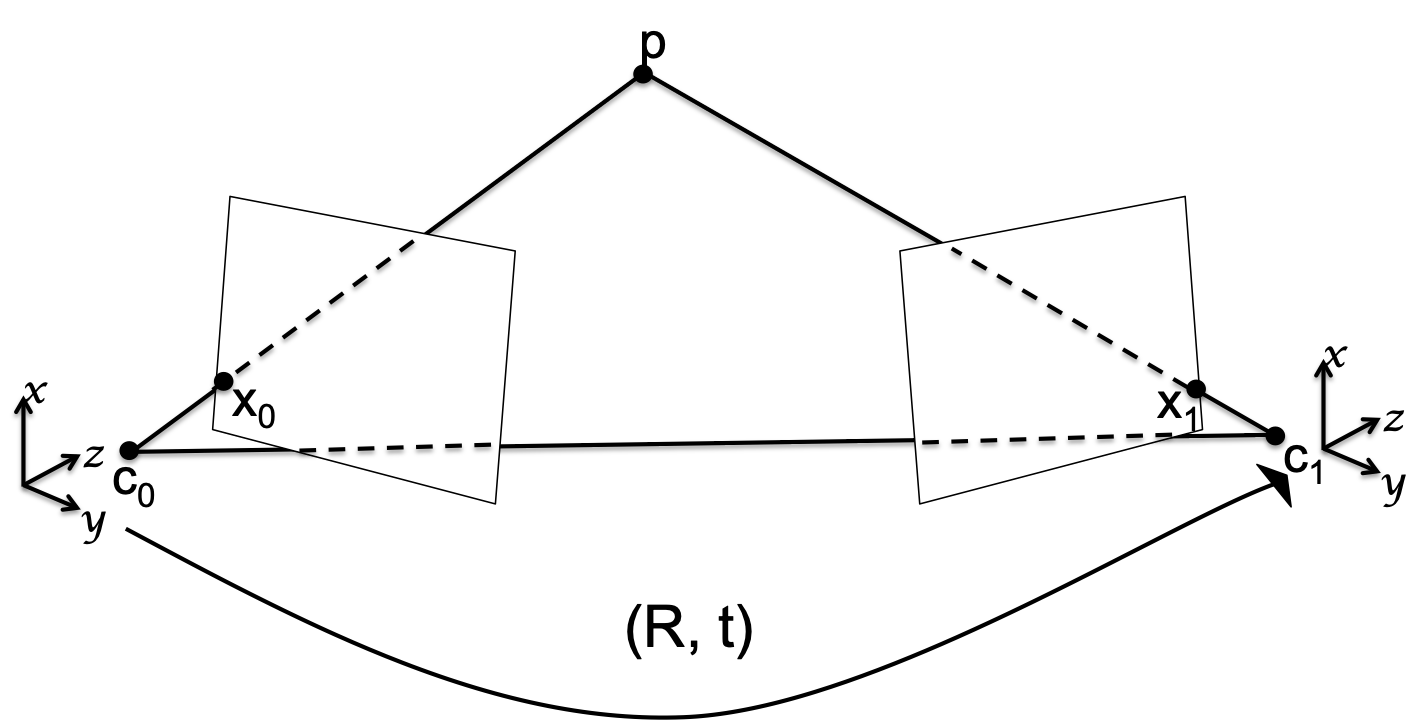
\includegraphics[width=\linewidth]{figures/two_view_camera_setup.png}
    \caption{A 3D point $\mathbf{p}$, projected on two image planes. Projected points have coordinate $\mathbf{x}_{0}, \mathbf{x}_{1}$. The two views are related by the rotation $R$ and translation $t$. }
    \label{fig:two_view_image}
\end{figure}
\newline
{\color{red}
\textbf{How a camera works:}
\newline
Essentially, a camera works by taking a point in 3D space and projecting it onto a 2D image (plane). A common mathematical model for this camera projection model is the perspective camera model. Under this model, a camera projection can be viewed as follows: 
\newline
Let $\mathbf{p} = [X,Y,Z]$ be a point in 3D space $\mathbb{R}^3$, then the 2D projection of this point via the camera is modeled via the equation:
\begin{equation}
    Z
    \begin{bmatrix}
        x \\
        y \\
        1
    \end{bmatrix}
    = K
     \begin{bmatrix}
        X \\
        Y \\
        Z
    \end{bmatrix}
    = K\mathbf{p}
\end{equation}
where $K \in \mathbb{R}^{3 \times 3}$, known as the camera matrix is generally of the form
\begin{equation*}
    \begin{bmatrix}
        fs_x  & fs_{\theta} & c_x \\
        0 & fs_y & c_y \\
        0 & 0 & 1
    \end{bmatrix},
\end{equation*} with the contents being physical properties of the camera. 
\newline
Here, $x,y$ are the coordinates of the projected point on the image plane. In what follows, we will denote $\mathbf{x} = [x,y,1]^{T}$. 

\textbf{Two views:}
\newline
\newline
When we have two views of the same point, we can think of it simply as the same point viewed by two cameras at different locations $c_1, c_2$.  The camera locations are related by the rigid motion $R, t$ where $R$ is a rotation matrix in SO(3) and $t$ is a translation vector $\mathbb{R}^3$.  SO(3) is the set of rotation matrices in $\mathbb{R}^{3 \times 3}$, i.e. the set of all orthonormal matrices with determinant = 1 in $\mathbb{R}^{3\times 3}$
\newline
\newline
% TODO, properties of rotation matrix
\textbf{Pose estimation:}
\newline
\newline
Putting both pieces together, we can derive an equation relating the coordinates of the projections of a point in both image planes.  We will also assume that both cameras have the same camera matrix, $K$. Let $\mathbf{x}_{0},\mathbf{x}_{1} $ be the coordinates of the projection of the 3D point $\mathbf{p}$ in camera views 0 and 1 respectively. We fix the global coordinate frame to be at the camera location in view 0, so that a point $\mathbf{p}$ in view 0 has coordinate $R\mathbf{p} + t$ in view 1. Then, we can write that: 
\begin{align}
    & Z_{1}\mathbf{x}_1 = K(R\mathbf{p} + t) = K(RZ_{0}K^{-1}\mathbf{x}_{0} + t) \\
    & \implies Z_{1}K^{-1}\mathbf{x}_{1} = RZ_{0}K^{-1}\mathbf{x}_{0} + t 
\end{align}
We assume that we know $K$, so we can write $K^{-1}\mathbf{x} = \tilde{\mathbf{x}}$ for any $\mathbf{x}$.
\begin{equation}
    \implies Z_{1}\tilde{\mathbf{x}}_1 = Z_{0}R\tilde{\mathbf{x}}_0  + t
\end{equation}

We may take the cross product of both sides with $t$, to obtain. 
\begin{equation}
    Z_{1}(t \times \tilde{\mathbf{x}}_1) = Z_{0}(t \times R\tilde{\mathbf{x}}_0 )
\end{equation}

Taking the dot product with $\tilde{\mathbf{x}}_{1}$,  and noting that the dot product of othorgonal vectors is zero, we obtain 
\begin{align}
Z_{1}{\tilde{\mathbf{x}}_{1}}^T(t \times &\tilde{\mathbf{x}}_1) = Z_{0}{\tilde{\mathbf{x}}_{1}}^T(t \times R\tilde{\mathbf{x}}_0 )\\
\implies 0 &= Z_{0}{\tilde{\mathbf{x}}_{1}}^T(t \times R\tilde{\mathbf{x}}_0 )\\
\implies 0 &= {\tilde{\mathbf{x}}_{1}}^T(t \times R\tilde{\mathbf{x}}_0 )\\
&= {\tilde{\mathbf{x}}_{1}}^T E\tilde{\mathbf{x}}_0. \label{eq:Epipolar_Constraint}
\end{align}
where we define $E=t\times R$.
}
\newline
\textbf{Problem setup:}
\newline
Given a point $\mathbf{p} \in \mathbb{R}^3$, and its projection to images in two views $\mathbf{\tilde{x}}_{0} = [\tilde{x}_0, \tilde{y}_0, 1]^T,\mathbf{\tilde{x}}_{1} = [\tilde{x}_1, \tilde{y}_1, 1]^T $ respectively, and asumming both views are related through a rotational matrix $R \in$ SO(3) (the 3D rotation group SO(3) is the group of rotation matrices [i.e. orthonormal and determinant $=1$] in $\mathbb{R}^{3\times 3}$, corresponding to rotations about the origin in $\mathbb{R}^3$) and translation vector $t \in \mathbb{R}^3$. The geometric relationship between the projections in the two views, is given by:
\begin{equation}
    {\tilde{\mathbf{x}}_{1}}^T E\tilde{\mathbf{x}}_0  = 0,
\end{equation}
where 
\begin{equation}
    E = [t]_{\times}R.
\end{equation}
\newline
\newline
The matrix $E = [t]_{\times}R$ is known as the \textit{essential matrix}. The cross product matrix $[t]_{\times}$ is a skew -symmetric matrix (i.e. $[t]_{\times}^\top=-[t]_{\times}$) representing the cross product of $t$ with any appropriately sized vector. It returns the $\mathbf{0}$ vector when pre- and post-multiplied by the same vector, since the cross product is orthogonal to its factors. Concretely, given a vector $t = [t_0, t_1, t_2]^T$,
\begin{equation}
t \times x = [t]_{\times}x
=
    \begin{bmatrix}
    0 & -t_{2} & t_{1} \\
    t_{2} & 0 & -t_{0} \\
    -t_{1} & t_{0} & 0
    \end{bmatrix}
    x
\end{equation} 
for any appropriately sized vector $x$.

\paragraph{1.1. Properties of the Essential Matrix:}\ 

A nonzero matrix $E \in \mathbb{R}^{3 \times 3}$ is said to be an essential matrix if and only if 
\begin{enumerate}
\item 
It has a singular value decomposition $E = U \Sigma V^{T}$, with 
\begin{equation*}
\Sigma = 
    \begin{bmatrix}
    \sigma & 0 & 0\\
    0 & \sigma & 0\\
    0 & 0 & 0
    \end{bmatrix}
\end{equation*}
\item
 and $U, V \in$ SO($3$), i.e. $U,V$ are rotation matrices. Note that in general, the $U,V$ matrices of an SVD are only required to be orthorgonal, the extra requirement here is the the det($U$) = det($V$) = 1, making $U,V$ rotation matrices.
 \end{enumerate}
 
 The space of matrices with the properties above is known as the \textit{essential space}.
 
 \paragraph{1.2. Estimating the Essential Matrix:}\ 
 
 The equation \eqref{eq:Epipolar_Constraint} is linear in $E$. To see this, given the projections $\mathbf{\tilde{x}}_{0}, \mathbf{\tilde{x}}_{1}$ of a point $\mathbf{p}$ in view 0 and view 1 respectively, where
 $\mathbf{\tilde{x}}_{0} = [\tilde{x}_0, \tilde{y}_0, 1]^T$ and $\mathbf{\tilde{x}}_{1} = [\tilde{x}_1, \tilde{y}_1, 1]^T$ and the essential matrix $E$ is written as 
 \begin{equation}
 E = 
     \begin{bmatrix}
     e_{11} & e_{12} & e_{13} \\
     e_{21} & e_{22} & e_{23} \\
     e_{31} & e_{32} & e_{33} 
     \end{bmatrix},
 \end{equation}
 
 we may re-write equation \eqref{eq:Epipolar_Constraint} as 
 $\mathbf{a}^{T}E^{s} = 0 $, with:
 \newline
 $\mathbf{a} = [\tilde{x}_{1}\tilde{x}_{2}, \tilde{x}_{1}\tilde{y}_{2}, \tilde{x}_{1}, \tilde{y}_{1}\tilde{x}_{2}, \tilde{y}_{1}\tilde{y}_{2}, \tilde{y}_{1}, \tilde{x}_{2}, \tilde{y}_{2}, 1]^T$
 \newline 
 $E^{s} = [e_{11},e_{21},e_{31},e_{12},e_{22},e_{32},e_{13},e_{23},e_{33}]^{T}$
 \newline
 \newline
 Given $n$ points $p_0, \hdots, p_{n-1}$ and their projections in both views, we may construct a system of linear equations:
 \begin{equation}\label{eq:Min_norm_approximation_of_essential_matrix}
   \mathcal{X}E^{s} = 0  
 \end{equation}
 
 with $\mathcal{X} \coloneqq [\mathbf{a}_{0},\mathbf{a}_{1},\hdots, \mathbf{a}_{n-1}]^{T}$. For the basic algorithm, we will need at least eight of these points. Once we have solved for $E^{s}$, we may rearrange to components to obtain $E$.
 
 In practice, due to noise in measurements of the points and their projections, $\mathcal{X}$ may not have a non-trivial nullspace and we will have to be satisfied with solving
 \begin{equation}\label{eq:Min_norm_approximation_of_essential_matrix2}
    \underset{E^{s}}{\text{min }} ||\mathcal{X}E^{s}||^{2}_2
 \end{equation}
 instead of \eqref{eq:Min_norm_approximation_of_essential_matrix}.
 In general, the solution to this minimization problem need not lie in the essential space --- once we find a solution $F$ to the above problem, we will need to project it onto the Essential Space.
 
\begin{enumerate}
\item{\textbf{Projection onto the Essential Space}}
    Given a matrix $F \in \mathbb{R}^{3 \times 3}$, with SVD $F = U\Sigma V^T$, and $U,V \in$ SO(3), find the solution $E^{*}$ to the following problem:
    \begin{equation}
        \underset{ E \in \mathcal{E}}{\text{argmin }} ||E - F||_{f}^{2}.
    \end{equation}
    
    Here $||.||_{f}$ is the Frobenius norm, and $\mathcal{E}$ is the essential space. You should assume that $ E^{*} = U \Sigma_{\sigma} V^{T}$, i.e. $F$ and $E^{*}$ share the same matrices $U,V\in$ SO(3) matrices. 
    
    \textit{Hint:} $\Sigma_{\sigma}$ should be of the form 
    \begin{equation*}
        \begin{bmatrix}
        \sigma & 0 & 0 \\
        0 & \sigma & 0 \\
        0 & 0 & 0
        \end{bmatrix}
    \end{equation*}
    \newline
    
    \sol{\input{3D_reconstruction/1.1.tex}}
    
\item{\textbf{Recovering the translation vector:}}
    Recall that $E = [t]_{\times}R$. Show that the translation vector $t$ is in the left null space of $E$. 
    \newline
    
\sol{\input{3D_reconstruction/1.2.tex}}
\item
    Unfortunately, we cannot say more than this, given just the essential matrix $E$. We may estimate the direction of $t$ as a unit norm vector in the left null space of $E$. In addition, this procedure gives us two solutions, since for any unit norm vector $\hat{t}$ in the left null space of $E$, $-\hat{t}$ is also a valid solution. Later we will see how to recover the proper sign. 
    \newline 
    \newline
    Write a procedure in the IPython notebook to recover the two directions of translation from the essential matrix $E$ using SVD. Normalize the resulting translation vector before returning it.
    \newline
    
    \sol{\input{3D_reconstruction/1.3.tex}}
    
\item{\textbf{Recovering the Rotation matrix:}}
    Next, we will attempt to recover the rotation between both views. Because we only know the estimate of the essential matrix up to sign, $\pm E$ are both solutions to our minimization problem \eqref{eq:Min_norm_approximation_of_essential_matrix2}, and also because typical SVD algorithms do not provide a guarantee that the $U,V$ matrices are rotation matrices, we will have four different solutions for our rotation matrix, from which only two will be true rotation matrices, i.e. det($R$) = 1. 
    
    Given an essential matrix of the form $E = U \Sigma V^T$, and defining 
    \begin{equation*}
        R_{Z}^T(\frac{\pi}{2}) = 
        \begin{bmatrix}
             0 & 1 & 0 \\
             -1 & 0 & 0 \\
             0 & 0 & 1 
        \end{bmatrix}, 
        R_{Z}^T(-\frac{\pi}{2}) = 
         \begin{bmatrix}
             0 & -1 & 0 \\
             1 & 0 & 0 \\
             0 & 0 & 1 
        \end{bmatrix},
    \end{equation*} we can obtain the four estimates for the rotation matrix $R$ as, 
    \begin{equation*}
        R = \pm U R_{Z}^T(\pm \frac{\pi}{2}) V^{T}.
    \end{equation*}.
    
    We choose the two $R$'s with positive determinants to be our estimates for $R$. We will see how to settle on the final answer later.  Write a procedure in the Ipython notebook to return the valid rotation matrices from a given essential matrix $E$.

    \sol{\input{3D_reconstruction/1.4.tex}}
    
\item{\textbf{Estimating 3D position from 2D matches: Triangulation}}

    Our next step is to estimate the 3D position of a point $\mathbf{p}$, given its projection onto the two views $\mathbf{x}_0 = [x_0, y_0, 1]^T, \mathbf{x}_1 = [x_1, y_1, 1]^T$, an estimate of the rotation $R$ and translation $t$ between the two views, and camera parameters in the camera matrix $K$ (recall that $K^{-1}\mathbf{x} = \tilde{\mathbf{x}}$. For clarity, $\mathbf{x}, \tilde{\mathbf{x}}$ are both projections of a 3D point, but in different units ).
    
    The full derivation of this solution is beyond the scope of this course; however, to obtain the 3D position of the point $\mathbf{p}$, we start by constructing the matrices
    \begin{equation}
        P_0 = K[I_{3\times 3},\mathbf{0}_{3 \times 1}] =
        \begin{bmatrix}
           \leftarrow P_{0}^{1T} \rightarrow \\
           \leftarrow P_{0}^{2T} \rightarrow \\
           \leftarrow P_{0}^{3T} \rightarrow \\
        \end{bmatrix}
        \in \mathbb{R}^{3 \times 4}, \hspace{5pt}
        P_1 = K[R,t] =
        \begin{bmatrix}
           \leftarrow P_{1}^{1T} \rightarrow \\
           \leftarrow P_{1}^{2T} \rightarrow \\
           \leftarrow P_{1}^{3T} \rightarrow \\
        \end{bmatrix}
        \in \mathbb{R}^{3 \times 4}.
    \end{equation}
    Note that the notation $P_{*}^{1T}, P_{*}^{2T}, P_{*}^{3T}$ are just the rows of $P_{*}$, they have nothing to do with  $\mathbf{p}$.
    \newline
    \newline
    Then we construct the matrix 
    \begin{equation}
        A = 
        \begin{bmatrix}
        x_0(P_{0}^{3T}) - P_{0}^{1T} \\
        y_0(P_{0}^{3T}) - P_{0}^{2T} \\
        x_1(P_{1}^{3T}) - P_{1}^{1T} \\
        y_1(P_{1}^{3T}) - P_{1}^{2T} \\
        \end{bmatrix}
        \in \mathbb{R}^{4 \times 4}.
    \end{equation}
    
    Then the following equation helps us find the 3D point $\mathbf{p}$
    \begin{equation}
        A
        \begin{bmatrix}
        \mathbf{p} \\
        1
        \end{bmatrix}
        = \mathbf{0}_{4 \times 1}.
    \end{equation}
    
    Here, we are simply looking for an element in the nullspace of $A$ with $1$ as the fourth component. To find $\mathbf{p}$, we may simply find a (non-trivial) element in the null space of $A$ , divide this vector by its 4th component and take the first 3 components of the resulting vector as $\mathbf{p}$.
    \newline
    \newline
    Write a procedure in your Ipython notebook to triangulate a point $\mathbf{p}$, given its projection onto both images $\mathbf{x}_0, \mathbf{x}_1$ an estimate of $P_0, P_1$.
    \sol{\input{3D_reconstruction/1.5.tex}}
    
\item 
    Now that you have completed the triangulation function, we will make use of it to select the optimal $R, t$ from the 4 different combinations (2 for $R$, and 2 for $t$) of $R,t$ we had previously. \newline
    \newline
    Essentially, we will triangulate a set of 3D points from the projections of those points and choose the combination of $R,t$ that gives us most points in front of the camera, i.e. the z-coordinates (in a camera system the z direction points outwards)  of the points are positive. False combinations would give us a lot of points behind the camera, but we wouldn't have been able to see those points if this was the case.
    \newline
    \newline
    We have written most of this function for you, but want you to choose the best combination of $R,t$ given a count of the number of points in front of the camera. Complete this part of the function in your IPython notebook. 
    \newline
    
    \sol{\input{3D_reconstruction/1.6.tex}}
    
\item{\textbf{Reconstructing a chair from two views}}
    \begin{figure}[!h]
    \centering
    \begin{subfigure}{.5\textwidth}
      \centering
      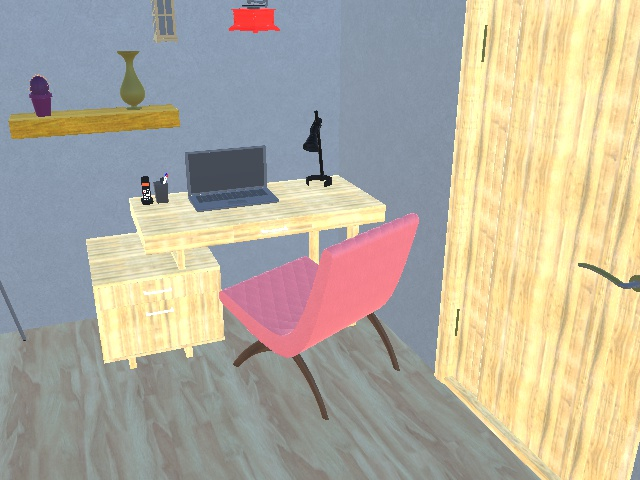
\includegraphics[width=\linewidth]{figures/view_0.jpg}
      \caption{View 0}
      \label{fig:sub1}
    \end{subfigure}%
    \begin{subfigure}{.5\textwidth}
      \centering
      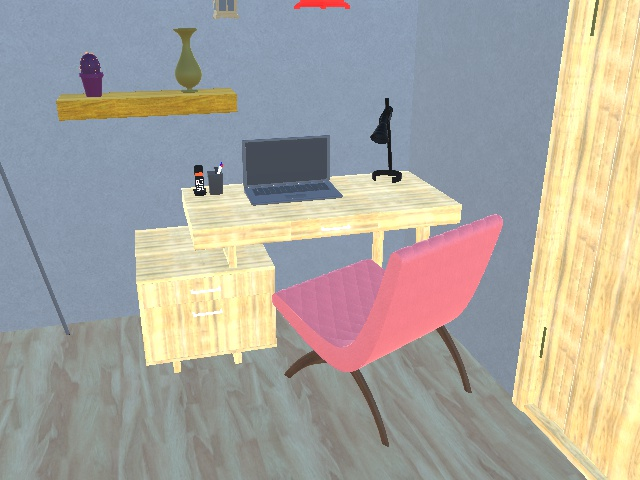
\includegraphics[width=\linewidth]{figures/view_1.jpg}
      \caption{View 1}
      \label{fig:sub2}
    \end{subfigure}
    \caption{Two views of the same scene}
    \end{figure}
    \newline
    \newline
    Finally, we are able to put all these ideas together to reconstruct an object. We have chosen to reconstruct the chair in the scenes below. Run all the cells of the Ipython notebook. Do you see a 3D chair? Take a screenshot  of the chair with all parts visible and attach to your write up.
    
    \sol{\input{3D_reconstruction/1.7.tex}}
\end{enumerate}

\newpage
\qns{Higher dimension least-square}

You are a world renowned animal specialist who has been studying the movement of animals to answer the pivotal question of our generation: can we approximate the movement of animals as a mathematical function? You controversially believe this is possible, and decide to test your hypothesis by observing the hunt of a tiger. You go to the best place to observe tigers, the Ranthambore National Park in Rajasthan, India, and set up a place where you can observe these majestic creatures hunt.

After a week in the wilderness, you have observed the tiger and realize that when it hunts, it moves according to a cubic function. However, your qualitative observations are insufficient if you are to convince the rest of the animal behavior scientists that your hypothesis holds true. You need to give them the exact function that describes how the tiger moves.

\begin{enumerate}
\item Luckily, you wrote down your exact observations of the tiger at 4 distinct points in the form of (x, y) coordinates, given below. As you know thanks to CS70, we have enough information to solve for a cubic polynomial. Using the points given, setup a system of linear equations in the form $\mathbf{A}\vec{x} = b$ that you can use to solve for the polynomial.
Hint: Any cubic function can be described as $ax^3 + bx^2 + cx + d$ for some $a, b, c, d$.

\begin{center}
 \begin{tabular}{c | c} 
 x & y \\ [0.5ex] 
 \hline
 1 & 8 \\ 
 2 & 12 \\
 3 & 10  \\
 4 & -4  \\
\end{tabular}
\end{center}

\newline
\sol{\item $g(x_1,x_2) = \dfrac{x_1^2}{4} + \dfrac{x_2^2}{9}$


}
\newline

\item Decompose the $\mathbf{A}$ matrix you constructed in the previous part using QR decomposition. How could you use this decomposition to solve for $\vec{x}$? Note: You may use a calculator (including Python or other scripting languages) to speed up algebraic work. Round to 3 decimal places and make sure to show your work. If using Python etc., please calculate everything explicitly (don't just call a library!).

\newline
\sol{\item Show that the following inequalities hold for any vector $x \in \Real{n}$:
\[
% \|x\|_\infty \le \|x\|_1 \le n \|x\|_\infty \\
% \|x\|_2 \le \|x\|_1 \le \sqrt{n} \|x\|_2 \\
% \|x\|_\infty \le \|x\|_2 \le\sqrt{n}\|x\|_\infty \\
\frac{1}{\sqrt{n}}\|x\|_2 \leq \|x\|_\infty \leq  \|x\|_2 \leq \|x\|_1 \leq \sqrt{n} \|x\|_2 \le n\|x\|_\infty.
\]

\textit{Hint:} For $\|x\|_1\leq \sqrt{n}\|x\|_2$, how might you express $\|x\|_1$ as the dot product of two vectors? Can you then use the Cauchy-Schwarz inequality to bound this dot product?}
\newline

Unfortunately, you need to leave the beauty of the wilderness and return to Berkeley for your EECS127 midterm (how inconvenient!). However, you would like to continue collecting data and work on your hypothesis remotely. So, you leave behind some sensors that can track the tiger hunt for you. Now that we have sensors, we have imperfect readings (because the sensors will have some noise and inaccuracies). Rather than take 4 exact measurements, we take many measurements to try to approximate the tiger's path.

\newline
\item How would you update your setup in part (a)? How can we solve this system?

\newline
\sol{\item $g(x) = \sin(x_1^2) \log (x_3 - x_2)$ where $x_i$ are scalars and $x_3 - x_2 > 0$.}
\newline

\item (Jupyter Notebook) Follow the instructions in the Jupyter notebook in order to solve the new system in part (c)

\newline
\sol{\item
\[
g(x) = \begin{bmatrix}
x_1^2/x_2 \\
\log(x_3) \sin(x_1/x_3)
\end{bmatrix}
\]}
\newline

\end{enumerate}
\newpage
\qns{Dynamical system as linear equation}

In this exercise, we consider a linear dynamical system as a matrix multiplication. We then apply our findings to compute the solution of the pendulum.

Let us consider the following dynamical system:
\[ \Dot{x} = A x + B u\]
with $u$ a control variable and $x$ the state of the system.

We want to approximate the solution $x(t)$ at time $t>0$, given $x(0)=x_0$.

We divided the time interval $[0, t]$ in $n$ time step of $\Delta t = \frac{t}{n}$: $[0, t/n], [t/n, 2t/n], \dots [(n-1)t/n, t]$.

We approximate the linear equation by:
$\frac{x_{k+1}-x_{k}}{\Delta t} = A x_k + B u$ where $x_k = x(k\Delta t)$ and $0\leq k <n$.

First we assume that $u = 0$, so $x_{k+1} = (A \Delta t + I) x_k$.

\begin{enumerate}
\item Assuming that $A$ is diagonalizable show that $\exists P,\ \lambda_1 \geq \dots \geq \lambda_m$, such that 
	\[ x_{k+1} = P \begin{bmatrix}
        1 + \lambda_1 \Delta t    &0       &\dots  &0\\
        0      &1 + \lambda_2 \Delta t     &       &\vdots\\
        \vdots &        &\ddots &0\\ 
        0      &\dots   &0      & 1 + \lambda_m \Delta t
    \end{bmatrix} P^{-1}  x_k
    \]

\sol{\item $g(x_1,x_2) = \dfrac{x_1^2}{4} + \dfrac{x_2^2}{9}$


}
\item Show that 
    \[  x(t) = P\begin{bmatrix}
        1 + \lambda_1 \frac{t}{n}    &0       &\dots  &0\\
        0      &1 + \lambda_2 \frac{t}{n}     &       &\vdots\\
        \vdots &        &\ddots &0\\ 
        0      &\dots   &0      & 1 + \lambda_m \frac{t}{n}
    \end{bmatrix}^n P^{-1} x_0
    \]

\sol{\item Show that the following inequalities hold for any vector $x \in \Real{n}$:
\[
% \|x\|_\infty \le \|x\|_1 \le n \|x\|_\infty \\
% \|x\|_2 \le \|x\|_1 \le \sqrt{n} \|x\|_2 \\
% \|x\|_\infty \le \|x\|_2 \le\sqrt{n}\|x\|_\infty \\
\frac{1}{\sqrt{n}}\|x\|_2 \leq \|x\|_\infty \leq  \|x\|_2 \leq \|x\|_1 \leq \sqrt{n} \|x\|_2 \le n\|x\|_\infty.
\]

\textit{Hint:} For $\|x\|_1\leq \sqrt{n}\|x\|_2$, how might you express $\|x\|_1$ as the dot product of two vectors? Can you then use the Cauchy-Schwarz inequality to bound this dot product?}
\item Show that, for $n\in \mathbb{N}$ big enough, $\forall a\in \mathbb{R}$, $(1+\frac{a}{n})^n = e^{n \ln (1+\frac{a}{n})}$. State the values of $n$ for which the equality is true.

\textit{Hint:} Recall that $\ln(x)$ is not defined for some value of $x$.

\sol{\item $g(x) = \sin(x_1^2) \log (x_3 - x_2)$ where $x_i$ are scalars and $x_3 - x_2 > 0$.}
\item Using the fact that $\ln (1+\frac{a}{n}) \sim \frac{a}{n}$ when $n\rightarrow\infty$, show that $\lim\limits_{n\rightarrow\infty}(1+\frac{a}{n})^n = e^a$.

\sol{\item
\[
g(x) = \begin{bmatrix}
x_1^2/x_2 \\
\log(x_3) \sin(x_1/x_3)
\end{bmatrix}
\]}
\item Show that 
    \[ \lim\limits_{n\rightarrow\infty} x(t) = P \begin{bmatrix}
        e^{\lambda_1 t}    &0       &\dots  &0\\
        0      & e^{\lambda_2 t}     &       &\vdots\\
        \vdots &        &\ddots &0\\ 
        0      &\dots   &0      & e^{\lambda_m t}
    \end{bmatrix} P^{-1}  x_0
    \]

\sol{\input{dynamical_system_solutions/5}}
\end{enumerate}

Now assume that $u\neq 0$. We are interested in the existence of an equilibrium point $x_{eq}$ such that $0 = Ax_{eq} + Bu$.

\begin{enumerate}
\setcounter{enumi}{5}
\item Show that an equilibrium point exists if and only if $\forall x\in N(A^\top),\ x^\top Bu = 0$.

\textit{Hint:} You might show first that if $Ax_{eq}=-Bu$ then $\forall x \in N(A^\top), x^\top Bu=0$. Then, you might use the fundamental theorem of linear algebra.

\sol{\input{dynamical_system_solutions/6}}
\item Let $u$ and $x_{eq}$ such that $0 = Ax_{eq} + Bu$. Let $x(0) = x_0$ and $\lambda_1<0$. Show that $\lim\limits_{t\rightarrow\infty}x(t) = x_{eq}$.

\sol{\input{dynamical_system_solutions/7}}
\end{enumerate}

Some applications. 
\begin{enumerate}
\setcounter{enumi}{7}
\item Let consider $A=(-1)$, $x_0 = 10$ and $u=0$, what is $x(t)$ (using e.)?

\sol{\input{dynamical_system_solutions/8}}
\end{enumerate}

\textbf{The pendulum}.

Let consider the following system: $\ddot{y} = -\omega^2 y $. 
Let $X = \begin{bmatrix}
    y \\ \dot{y}
\end{bmatrix}$.
We have that 
$\dot{X} = \begin{bmatrix}
    \dot{y} \\ \ddot{y}
\end{bmatrix}$.
\begin{enumerate}
\setcounter{enumi}{8}
\item Give $A$ a $2\times 2$ matrix such that $\dot{X} = A X$.
Also, write the matrix in the notebook ``Dynamical system.ipynb''.

\sol{\input{dynamical_system_solutions/9}}
\item Assume that $\lambda$ is an eigenvalue of $A$, show that it implies that $\lambda^2=-\omega^2$.

\sol{\input{dynamical_system_solutions/10}}
\end{enumerate}

We can diagonalize matrices in $\mathbb{C}$. For this specific case of $A$ then $\lambda_1 = j\omega$ and $\lambda_2 = -j\omega$. Also, the result of question e. is still true and $e^{j\omega t} = \cos(\omega t) + j \sin(\omega t)$. The solution of the system is $y = y_0 \cos(\omega t) + \frac{\dot{y}_0}{\omega} \sin(\omega t)$

\begin{enumerate}
\setcounter{enumi}{10}
\item Complete this question in the notebook by filling in $X$ in terms of $n$, $t$, $X_0$, and the eigenvalues/eigenvectors of $A$.

\sol{\input{dynamical_system_solutions/11}}

\item[Bonus.] With respect to this exercise explain the quote of Iron Man in Avengers Endgame: ``the singular value decomposition of the inverted Mobius strip will give you an eigenvalue that will bring you back in the past.''

\sol{\input{dynamical_system_solutions/bonus}}
\end{enumerate}

\end{qunlist}
\end{document}
